\section{Verfahrensentwicklung}


Das im vorhergehenden Kapitel entwickelte Tool soll im Folgenden zunächst am Beispiel einer Flächenanalyse der Stadt Karlsruhe getestet werden, da im Gegensatz zur Verkehrssituation für diesen Fall genaue Vergleichsdaten vorliegen. Es werden die für die Untersuchung entscheidenden Parameter ermittelt und deren Einfluss auf die entsprechenden Größen untersucht. Im Anschluss daran wird in einem zweiten Abschnitt ein standardisiertes Vorgehen vorgestellt, welches zur systematischen Verkehrsanalyse verschiedener Städte und Gebiete verwendet werden soll.

% a) Kalibrierung und Sensitivitätsanalyse
\subsection{Kalibrierung und Sensitivitätsanalyse}

Das entwickelte Tool wird zunächst auf das Gebiet des Stadtgebiets Karlsruhe angewendet. Der Stadtkreis Karlsruhe umfasst laut Statistischem Landesamt Baden-Württemberg (Stand 2015) eine Fläche von rund \num{17.346} \si{\hectare} \cite{StatBaWu_Flaeche}, die Einwohnerzahl beläuft sich auf \num{307755} \cite{StatBaWu_Einw}.\\
Es gilt zu zeigen, dass das Verfahren die reale Flächenaufteilung im Stadtgebiet abbilden kann. Hierbei verfolgt google maps eine eigene Klassifizierung der Flächennutzungen, die sich nicht mit den sogenannten "\textit{tatsächlichen Nutzungsarten}" der  \textit{Arbeitsgemeinschaft der Vermessungsverwaltungen der Länder der Bundesrepublik Deutschland (AdV)}, welche die Grundlage aller deutschen Liegenschaftskataster bilden, deckt \cite{advnutz}. Als Vergleichsbasis wird im Folgenden zunächst der Anteil an Naturfläche gewählt, da dieser in den Klassifizierungen der AdV und in denen von google maps ähnlich definiert ist.\\ 
\newline
Zunächst wird untersucht, welche Zoomstufe in google maps sinnvollerweise ausgewählt werden muss, um das Stadtgebiet darstellen und analysieren zu können. Bei der Entscheidung, mit welcher Zoomstufe gearbeitet werden soll, gilt es, zwischen den Genauigkeitsanforderungen  der Daten und einer akzeptablen, zu verarbeitenden Datenmenge abzuwägen. Hierbei gelten die folgenden beiden Einschränkungen:
\begin{itemize}
\item Einerseits sollte das erzeugte Analysegebiet möglichst wenig über die Grenze des Stadtgebiets hinausragen, da die Analyse der Flächennutzung sonst verfälscht wird. Im vorliegenden Fall kann die minimale Zoomstufe damit zu 12 festgelegt werden, wie Abbildung \ref{fig:Stadtgebiet_KA} zeigt, da in diesem Fall das gesamte Stadtgebiet auf nur einer Kachel dargestellt werden kann.
\item Auf der anderen Seite wird die maximale Zoomstufe von google je nach Datengrundlage vorgegeben, in Karlsruhe ist die maximale Zoomstufe mit 21 gegeben. Wie Abbildung \ref{fig:Schloss_KA} am Beispiel des Karlsruher Schlosses darstellt, führt dies auf eine Darstellung auf Gebäudeebene. Eine solch hohe Diskretisierung liefert zwar eine äußert präzise Darstellung der städtischen Flächen, ist aus Gründen des Speicher- und Rechenaufwandes nicht sinnvoll, da zur Darstellung des Stadtgebietes in diesem Fall mehrere 10.000 Einzelkacheln analysiert werden müssten.
\end{itemize}
Um das gesamte Stadtgebiet mit hoher Präzision abbilden zu können und gleichzeitig eine adaptive Anpassung der Kachelauswahl an die Stadtgrenze zu ermöglichen, wird in der vorliegenden Kalibrierung mit einer (vergleichweise hohen) Zoomstufe von 17 gearbeitet. Auch hier wird für das Stadtgebiet Karlsruhe bereits die Analyse von knapp 1500 Einzelkacheln notwendig, weswegen für die spätere Anwendung eine geringere Zoomstufe empfohlen wird.\\
\newline
%
\begin{figure}
  \centering
    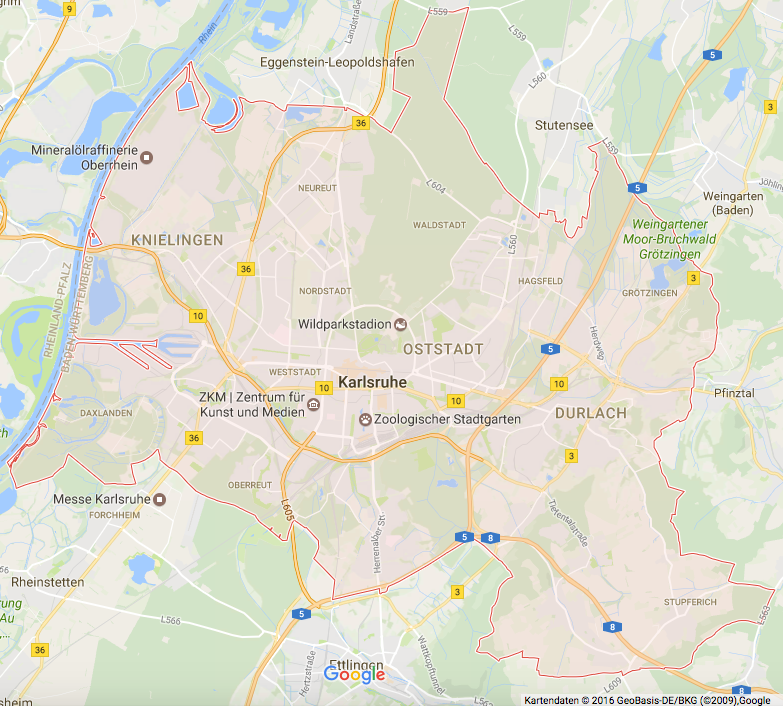
\includegraphics[width=0.55\textwidth]{images/3_Stadtgebiet_KA_zoom12.png}
    \caption{Darstellung der Gemarkungsgrenze des Stadtkreises Karlsruhe [Quelle: google maps, Zoomstufe 12]}
    \label{fig:Stadtgebiet_KA}
\end{figure}
%
\begin{figure}
  \centering
    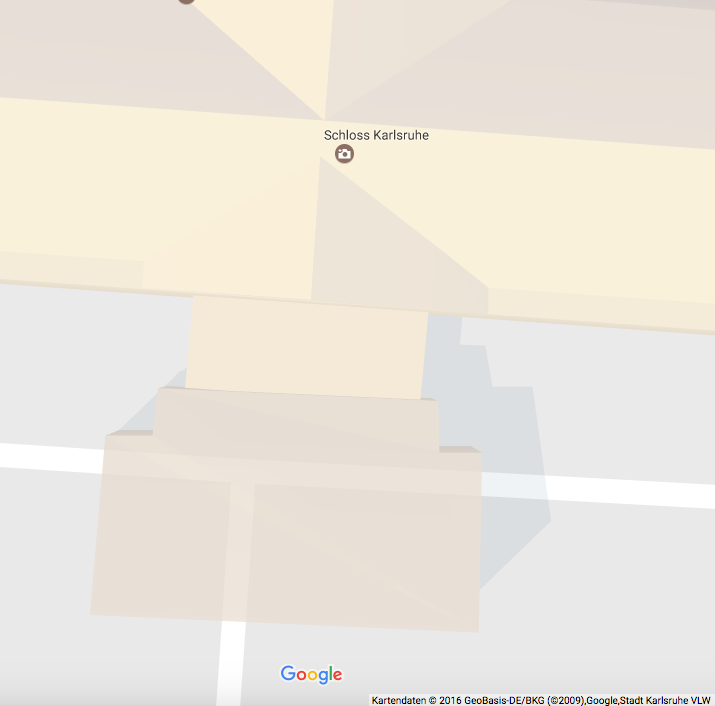
\includegraphics[width=0.6\textwidth]{images/3_KA_Schloss_zoom21.png}
    \caption{Darstellung des Karlsruher Schlosses bei höchster verfügbarer Zoomstufe [Quelle: google maps, Zoomstufe 21]}
    \label{fig:Schloss_KA}
\end{figure}
%
Da google maps die wählbaren Zoomstufen nicht mit einem festen kartographischen Maßstab verknüpft, muss dieser durch eigene Abstandsmessungen ermittelt werden. Bei Zoomstufe 17 besitzt eine der erzeugten quadratischen Einzelkacheln beispielsweise eine Kantenlänge von ca. \num{500} \si{\metre}, wie in Abbildung \ref{fig:Zoomvgl} zu sehen ist.\\
%
\begin{figure}
  \centering
    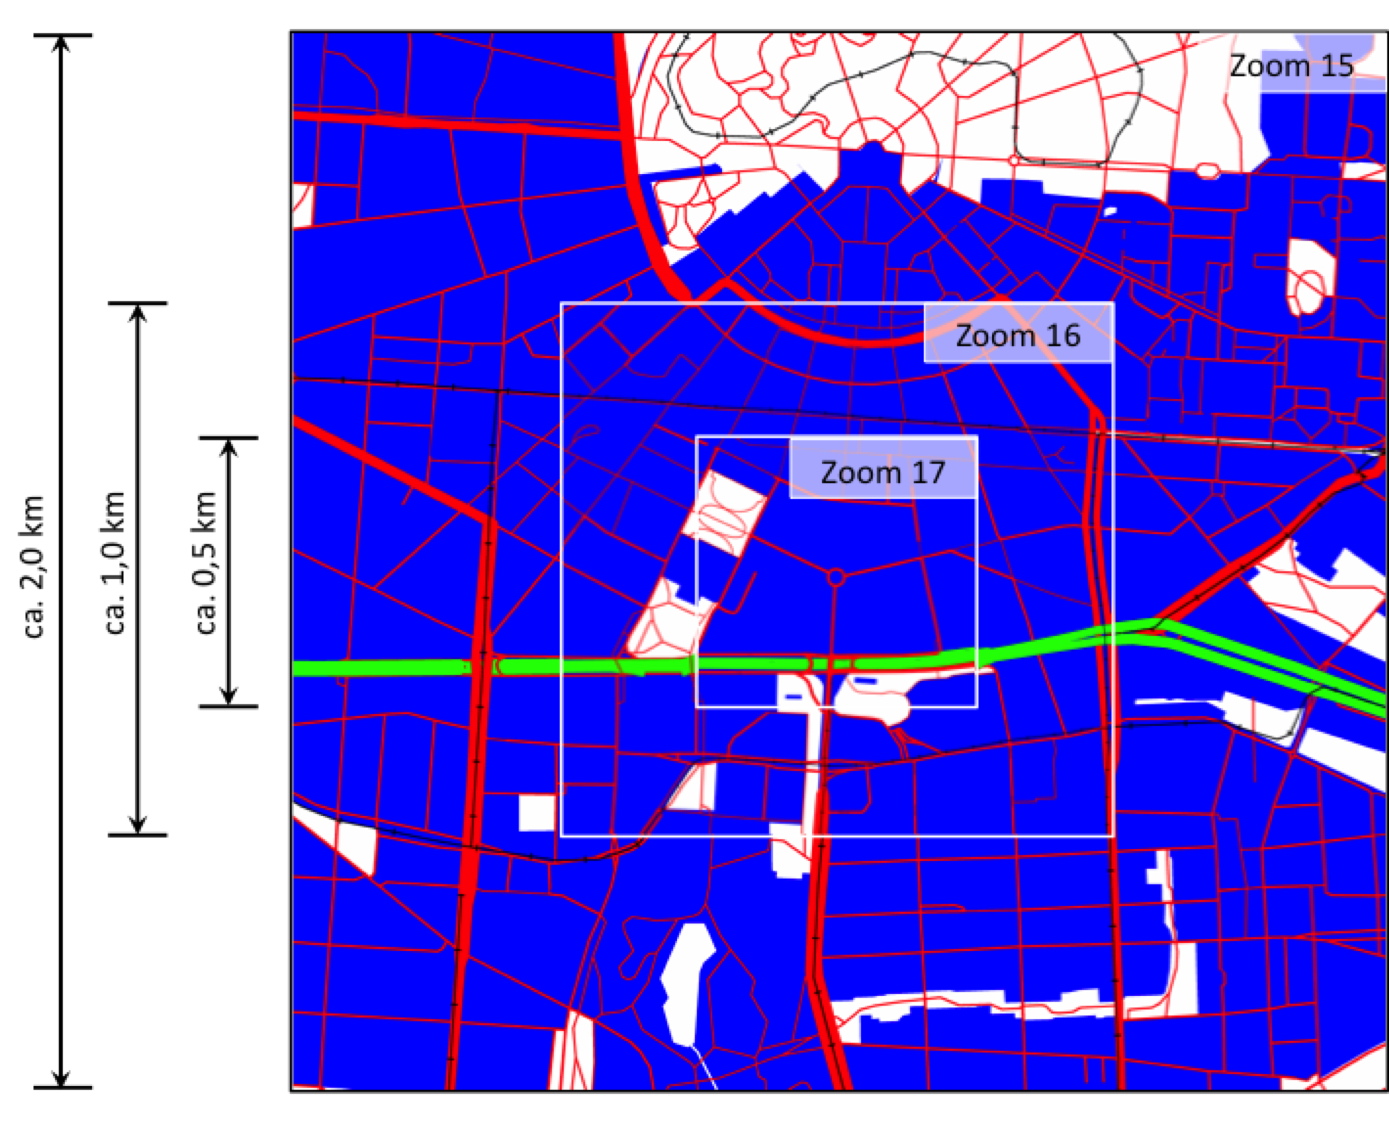
\includegraphics[width=0.6\textwidth]{images/3_Zoomvergleich_KA.png}
    \caption{Vergleich der Kachelabmessungen bei verschiedenen Zoomstufen}
    \label{fig:Zoomvgl}
\end{figure}
%
%
\newline
\begin{figure}
  \centering
    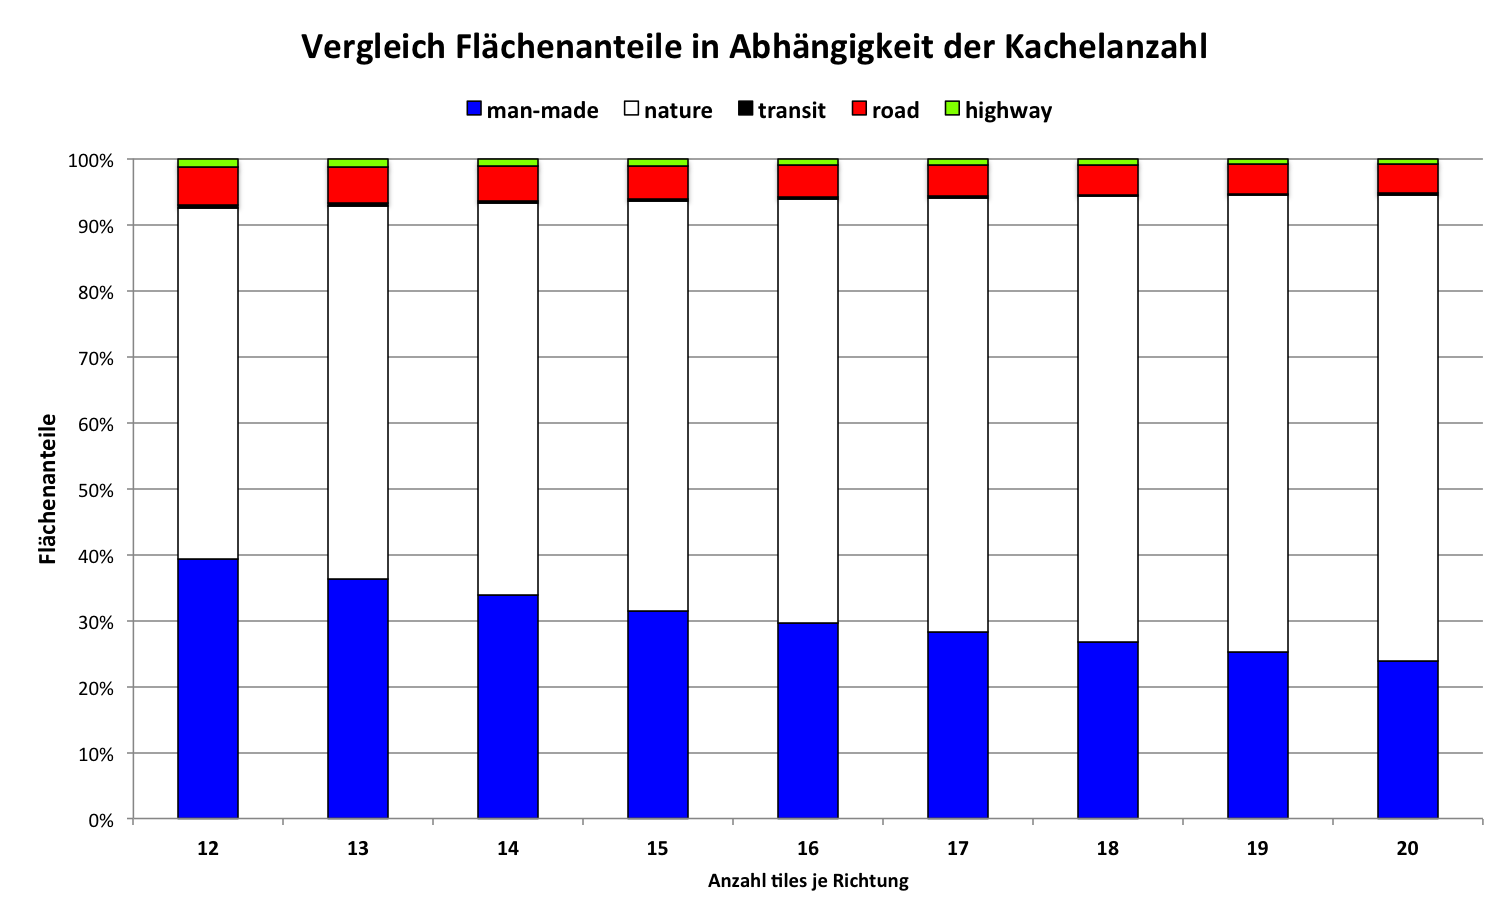
\includegraphics[width=0.92\textwidth]{images/3_Kachelvergleich_KA.png}
    \caption{Ergebnisse der Flächenanalyse für den Stadtkreis Karlsruhe für verschiedene Kachelanzahlen}
    \label{fig:Kachel_vgl}
\end{figure}
%
Im Weiteren wird die Flächenanalyse nun für verschiedene Anzahlen an Kacheln durchgeführt, um zu untersuchen, wie sich die Flächenanteile mit zunehmendem Einzugsgebiet der Analyse verändern. Die Ergebnisse der Flächenanalyse für die Eingabe an Tiles je Richtung zwischen 12 und 20 ist in Abbildung \ref{fig:Kachel_vgl} dargestellt.\\
Mit steigender Kachelzahl wird immer mehr des Stadtrandes und des Umlandes in die Analyse einbezogen, die Anteile von Verkehrsflächen und \textit{man-made area} an der Gesamtfläche sinken ab zu Gunsten der Naturflächen, welche bei  \((n:=15)\) (Kantenlänge des Analysequadrates ca. \num{14.5} \si{\kilo\metre}) und  \((n:=16)\) (Kantenlänge des Analysequadrates ca. \num{15.5} \si{\kilo\metre}) mehr als \num{60} \% einnehmen. Die zuletzt erwähnten Kachelanzahlen erzeugen ein Analysequadrat, welches in seinen Ausdehnungen in der Größenordnung des Stadtgebiets liegt. Für eine vollkommene Umschließung des Stadtgebiets (maximale Nord-Süd-Ausdehnung ca. \num{16.5} \si{\kilo\metre}), maximale Ost-West-Ausdehnung ca. \num{19.0} \si{\kilo\metre}) muss für die Anzahl an Kacheln \((n:=20)\) gewählt werden.\\
\newline
Allerdings muss erwähnt werden, dass die in Abbildung \ref{fig:Stadtgebiet_KA} dargestellte Gemarkung durch eine solche quadratische Analysefläche nur unzureichend angenähert werden kann. Dies zeigt ein Vergleich der Analyseergebnisse mit den Werten des Statistischen Landesamtes: hier wird der Anteil von Naturflächen mit ca. \num{52} \% angegeben, während die Analyse ca. \num{70} \% berechnet. Diese Überschätzung kann darauf zurückgeführt werden, dass bestimmte Bereiche wie beispielsweise große natürliche und landwirtschaftliche Bereiche in der Analyse erscheinen, obwohl sie nicht zum Stadtgebiet Karlsruhe gehören.\\
%
\begin{figure}
  \centering
    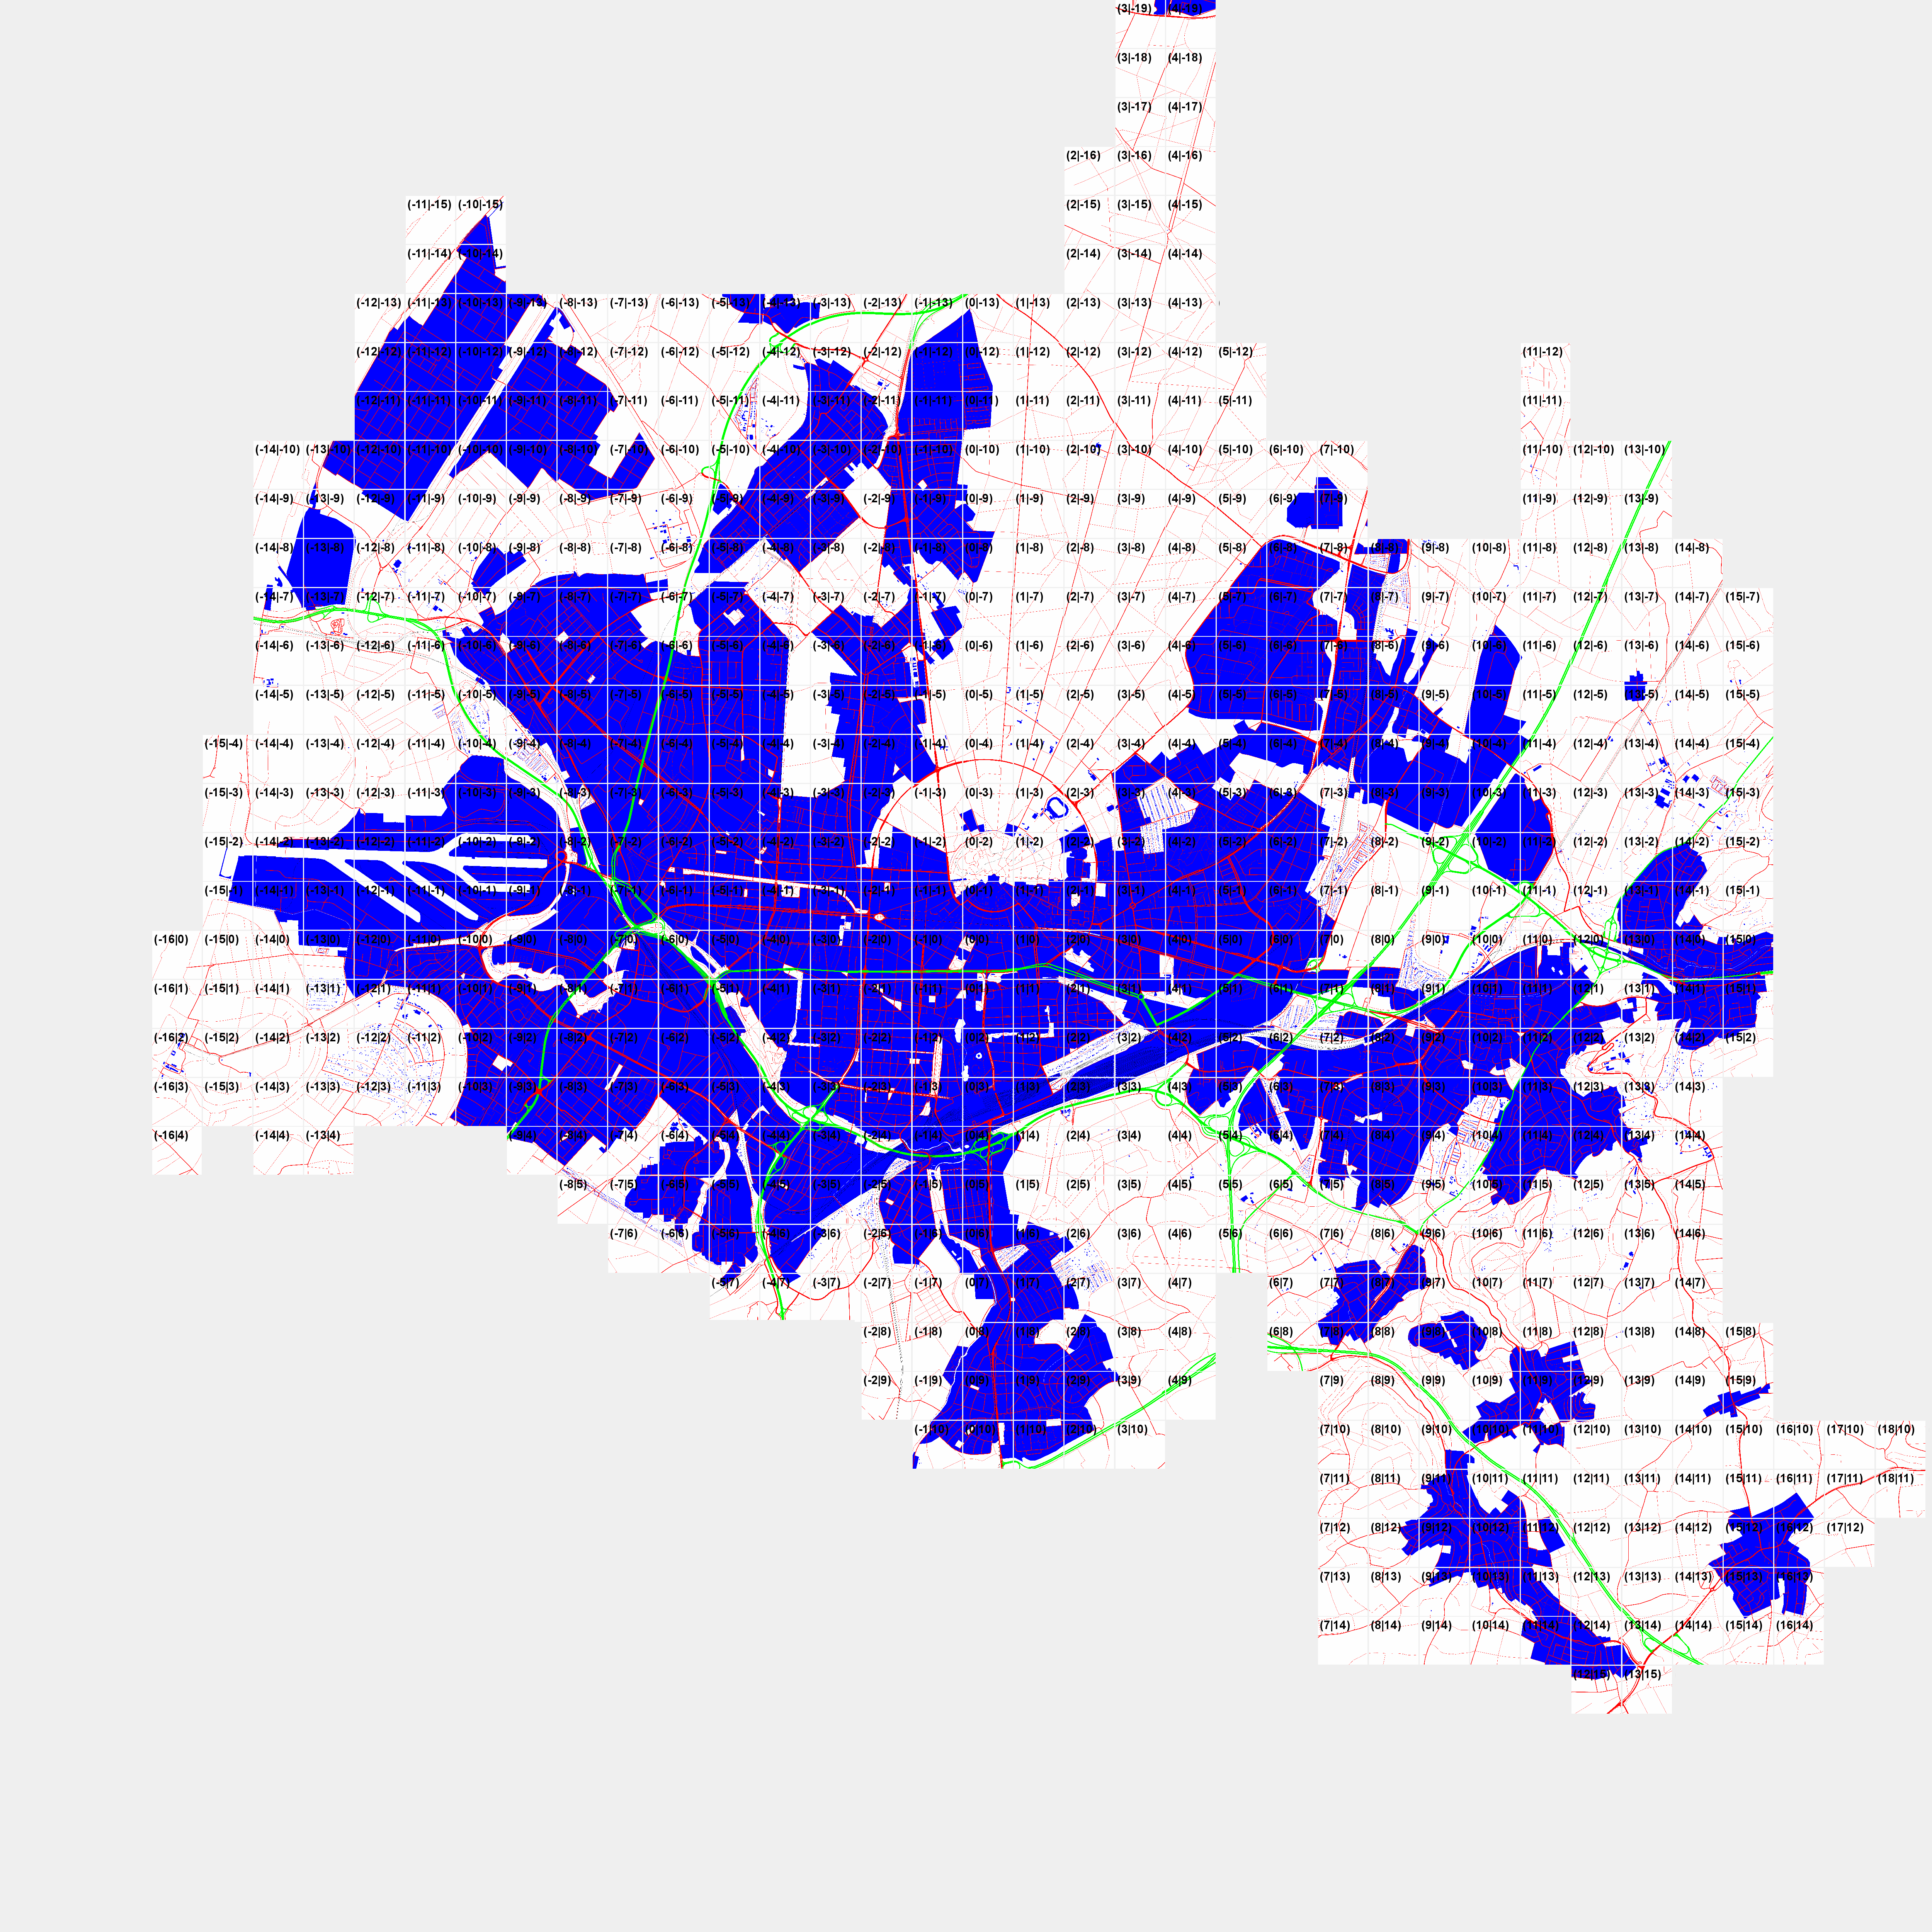
\includegraphics[width=0.9\textwidth]{images/3_KA_Kacheln_skip_ohne_zahlen.png}
    \caption{Darstellung der ausgewählten Kacheln zur genaueren Approximation der Karlsruher Stadtgrenze}
    \label{fig:Karlsruhe_skip_tiles}
\end{figure}
%
%
\begin{figure}
  \centering
    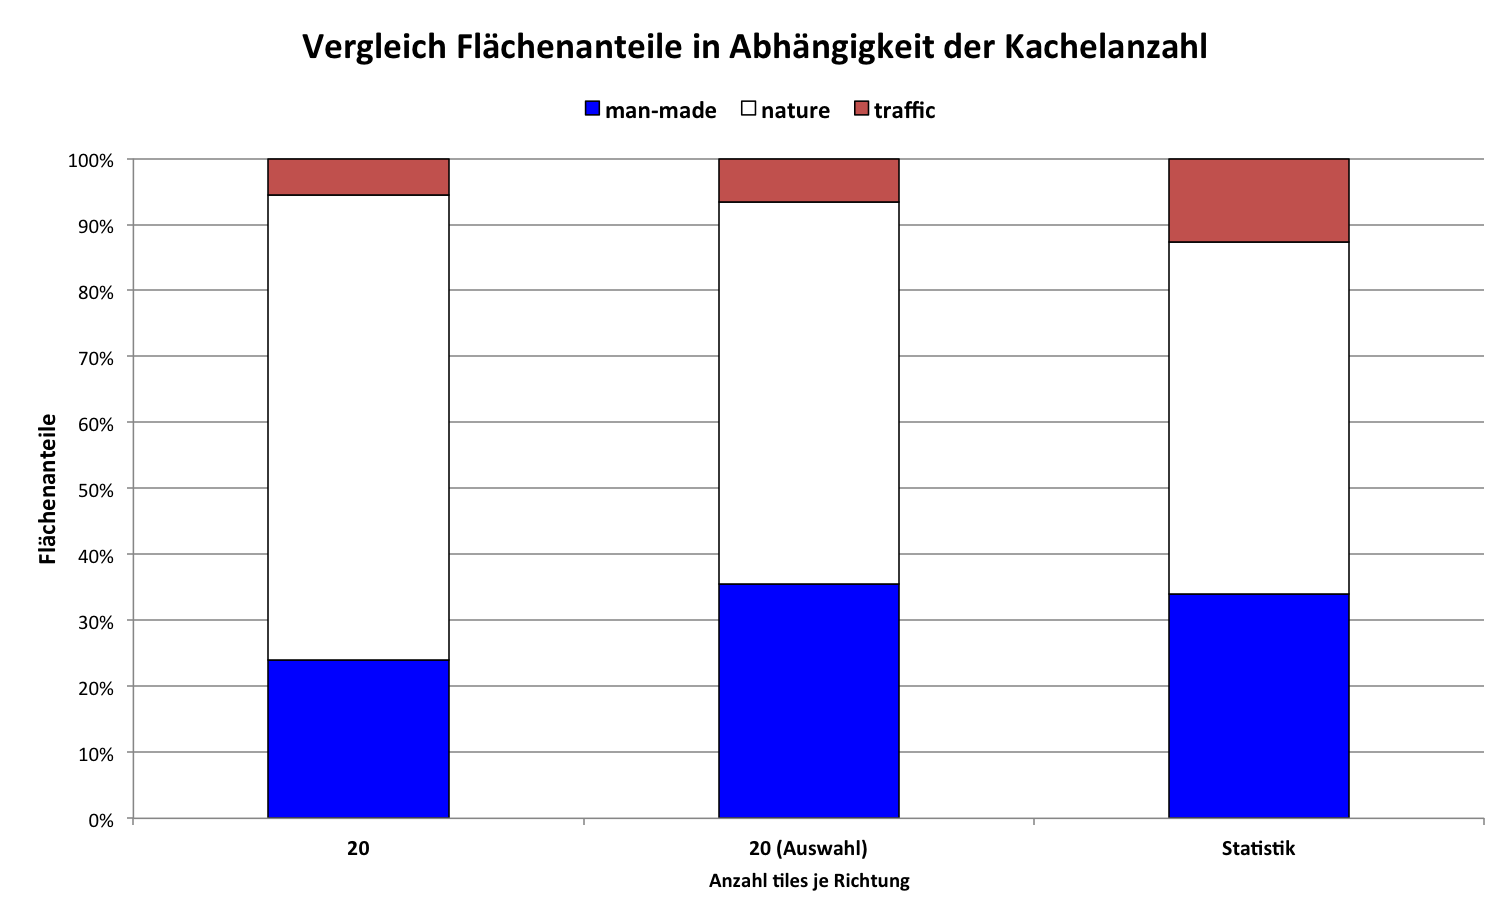
\includegraphics[width=0.92\textwidth]{images/3_Kachelvergleich_KA_skip.png}
    \caption{Ergebnisse der Flächenanalyse für den Stadtkreis Karlsruhe mit und ohne Kachelauswahl im Vergleich zu den statistischen Daten}
    \label{fig:Kachel_skip_vgl}
\end{figure}
%
%
\begin{figure}
  \centering
    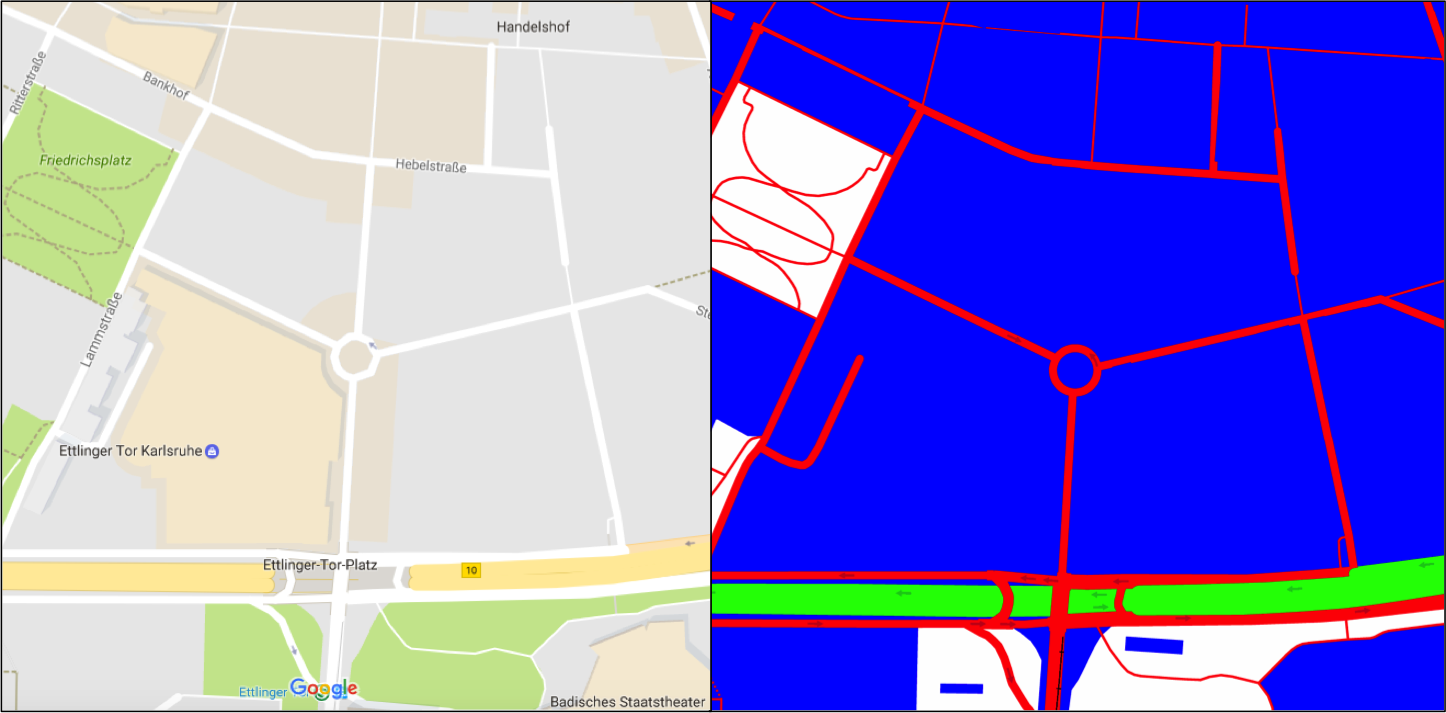
\includegraphics[width=0.85\textwidth]{images/3_google_Einstufung_Nutzung.png}
    \caption{Darstellung einer Straße in der Web-Ansicht (links) und Einstufung als man-made area nach dem Download (rechts)}
    \label{fig:versch_nutz_einstuf}
\end{figure}
%
Eine bessere Approximation kann durch gezielte Auswahl bzw. gezieltes Ausschließen einzelner Kacheln erreicht werden. Im Folgenden werden daher aus der Berechnung, die auf einer Kachelanzahl \((n:=20)\) basiert, diejenigen Kacheln ausgeschlossen, die außerhalb des Stadtgebietes liegen, sodass die übrigen die Stadtgrenze bestmöglich approximieren. Eine Darstellung der gewählten Kacheln findet sich in Abbildung \ref{fig:Karlsruhe_skip_tiles}. Dadurch verringert sich die Gesamtzahl der analysierten Kacheln von  ursprünglich \(1521\) auf nun \(680\). Das Resultat der Berechnung mit selektiertem Analysegebiet ist in Abbildung \ref{fig:Kachel_skip_vgl} den Ergebnissen der Berechnung mit vollen \(1521\) Kacheln sowie den aufbereiteten Daten des Landesamtes gegenübergestellt. Hierbei ist zu beachten, dass im Gegensatz zur bisherigen Benennung die Kategorien \textit{roads}, \textit{highway} sowie \textit{transit} in dieser Darstellung zur Oberkategorie \textit{traffic} zusammengefasst wurden, um eine Vergleichbarkeit der Berechnungsergebnisse mit den statisitschen Daten, welche einer anderen Klassifizierung folgen, zu ermöglichen. Während die Flächenanteile der Kategorie \textit{man-made} in der Berechnung um weniger als  \num{2} \% von denen des statistischen Landesamtes abweichen, zeigt sich bei Verkehrsflächen respektive Naturflächen eine Abweichung von rund \num{5} bis \num{6} \%. Letzteres kann unter anderem auf die unterschiedlichen Einstufungen der Flächen als Siedlungs- oder als Verkehrsfläche zurückgeführt werden. Ein Beispiel hierfür ist der Bereich um das Ettlinger Tor in Karlsruhe, der in Abbildung \ref{fig:versch_nutz_einstuf} dargestellt ist: Während in der Webansicht von google maps (links) in Kachelmitte eine in Nord-Süd-Richtung verlaufende Straße zu erkennen ist, wird diese von google tatsächlich, wie sich bei der Analyse (rechts) zeigt, als \textit{man-made area} eingestuft.\\

% b) Leitfaden zur Verkehrsanalyse
\subsection{Leitfaden zur Verkehrsanalyse}
Nachdem anhand des Beispiels Karlsruhe gezeigt worden ist, dass das entwickelte Verfahren zur Flächenanalyse die tatsächliche Flächennutzungen sehr gut darstellen kann, soll dessen Anwendung im weiteren Verlauf der Untersuchung bei einer Auswahl von Städten durchgeführt werden.\\
\newline
Das im Folgenden beschriebene Vorgehen stellt eine allgemeine Empfehlung für den Aufbau einer Verkehrsanalyse dar. Dessen Anwendung wird im Einzelfall sowohl von der Stadtgeometrie bzw. der Topograhpie der Region als auch von der Fragestellung bzw. Zielsetzung der Untersuchung maßgeblich beeinflusst. Daher ist es zielführend, vor Anwendung des folgenden Schemas in einer kurzen Voruntersuchung das Untersuchungsgebiet festzulegen und die gewünschten Zielgrößen zu definieren.
\begin{enumerate}
\item \textbf{Festlegen des Zentrums für die Kachelauswahl:} Im ersten Schritt muss ein geographischer Punkt als Zentrum für die Kachelauswahl gewählt werden. Dies kann der (zentrale) Punkt sein, den die Web-Anwendung google maps bei Eingabe des Stadtnames im Suchfeld ausgibt. In vielen Fällen ist es aber sinnvoller, den Punkt unabhängig davon möglichst mittig im bestimmten  Untersuchungsgebiet zu wählen, um die Anzahl an Kacheln, die zur vollständigen Überdeckung des Untersuchungsgebietes notwendig sind, gering zu halten. In speziellen Fällen, in denen beispielweise nur ein kurzer Streckenabschnitt zu analysieren ist, muss der zentrale Punkt ohnehin frei gesetzt werden. Die Koordinaten des Punktes sind im Format (\textit{latitude}, \textit{longitude}) anzugeben.
%
\begin{figure}
  \centering
    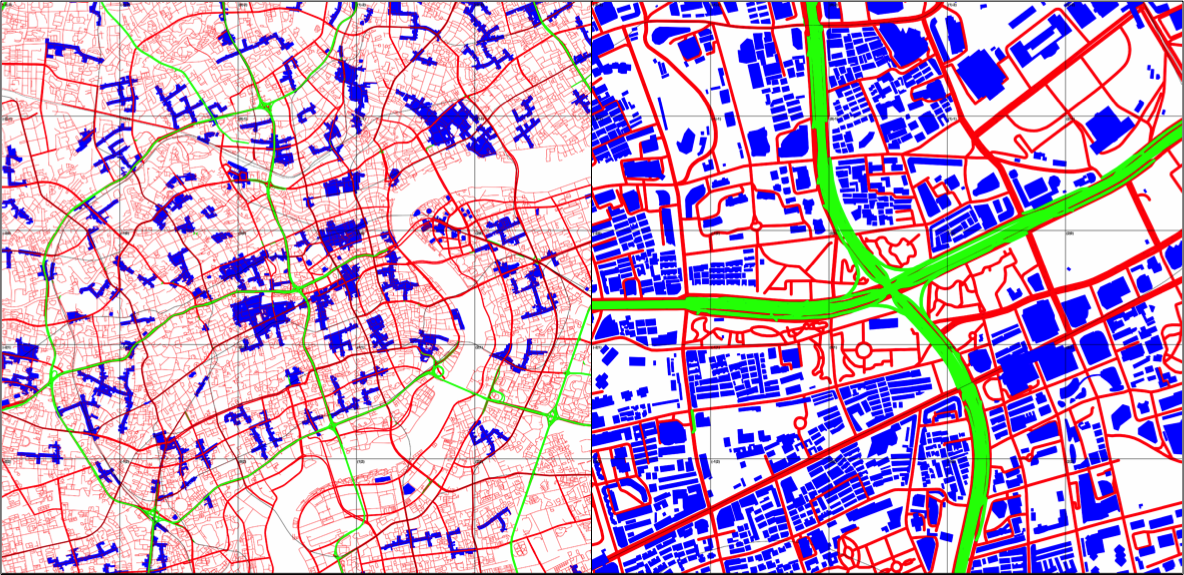
\includegraphics[width=0.92\textwidth]{images/3_Shanghai_Problem_Datenaufloesung}
    \caption{Darstellung des Stadtzentrums von Shanghai bei Zoomstufe 15 (links) und 18 (rechts); (links Darstellungsfehler aufgrund sehr detaillierter Gebäudeumrisse)}
    \label{fig:Fehler_Shanghai}
\end{figure}
%
%
\begin{figure}
  \centering
    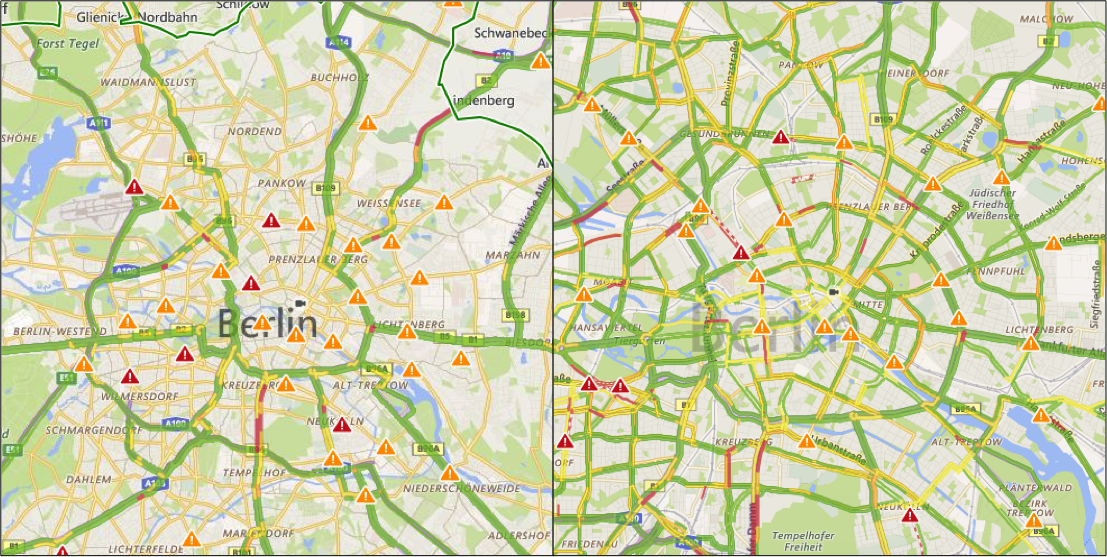
\includegraphics[width=0.92\textwidth]{images/3_bing_Aufloesung_traffic}
    \caption{Darstellung des Stadtzentrums von Berlin in verschiedenen Zoomstufen zeigt das Straßennetz in verschiedener Detaillierung}
    \label{fig:Fehler_Berlin}
\end{figure}
%
\item \textbf{Festlegen der Zoomstufe:} Im zweiten Schritt muss die Zoomstufe für die Kacheln festgelegt werden. Wie oben bereits beschrieben wurde, gilt es hierbei zwischen der Auflösegenauigkeit und dem steigenden Rechenaufwand abzuwägen. Daneben kann aber auch die lokal vorliegende Datengrundlage einen entsprechenden Einfluss auf die mögliche Zoomstufe besitzen. Bei den Flächendaten einerseits zeigt sich bei sehr präzisen Geodaten, dass google maps bei zu niedriger Zoomstufe die hochaufgelösten Daten zum Teil nicht mehr ordnungsgemäß abbilden kann und aus diesem Grund die bebauten Flächen falsch zuordnet. Ein Beispiel hierfür ist in Abbildung \ref{fig:Fehler_Shanghai} zu sehen: das Zentrum von Shanghai wird bei Zoomstufe 15 zu weiten Teilen als Naturfläche (Farbe weiß) eingestuft, die Gebäudeumrisse werden erst bei Zoomstufe 18 deutlich. Andererseits zeigt sich, dass bei den Verkehrsdaten kleinere Straßen bei zu niedriger Zoomstufe nicht dargestellt werden, obwohl sie mit Verkehrsinformationen belegt sind. Dies ist am Beispiel des Stadtzentrums von Berlin in Abbildung \ref{fig:Fehler_Berlin} dargestellt. Um die beiden genannten Probleme zu vermeiden empfiehlt es sich, verschiedene Zoomstufen im Hinblick auf deren Auflösegenauigkeit und ggf. auftretende Fehldarstellungen zu testen und die erzeugten Resultate zu vergleichen.
%
\item \textbf{Einstellung Anzahl Tiles:} Im folgenden Schritt wird die Anzahl der Tiles ausgewählt. Hierbei ist im Wesentlichen darauf zu achten, dass einerseits das Untersuchungsgebiet durch das Kachelraster vollständig abgedeckt wird, gleichzeitig aber die Gesamtzahl möglichst begrenzt bleibt. Kann hierbei kein zufrieden stellender Kompromiss zwischen beidem erzielt werden, müssen die in den vorhergegangen Schritten festgelegten Werte ggf. geändert werden. Die Begrenzung der Kachelanzahl ist besonders im Falle der Verkehrsdaten von entscheidender Wichtigkeit, da die Downloadraten durch die Anbieter des Kartenmaterials begrenzt sind und so nur eine bestimmte maximale Anzahl an Kacheln je Zeiteinheit analysiert werden kann. Ist die Gesamtzahl der Kacheln zu groß, kann der gewählte Zeitschritt der Analyse unter Umständen nicht mehr eingehalten werden.  
%
\item \textbf{Auswahl zu überspringende Tiles:} Abschließend können noch einzelne Tiles aus der Analyse ausgeschlossen werden. Hierzu zählen unter anderem Bereiche, die entweder keinen Einfluss auf die Analyse besitzen (z. B. reine Naturflächen) oder die im Rahmen der Untersuchung bewusst ausgeklammert werden (z. B. vorbeiführende Fernstraße soll aus der Stadtanalyse ausgeschlossen werden). Hierzu werden die auszuschließenden Kacheln einfach über die Indizes, welche ihren Platz innerhalb des Kachelrasters festlegen, angegeben.
\end{enumerate}



